\documentclass[12pt, a4paper]{article}

\usepackage{amsmath}
\usepackage{graphicx}

\begin{document}
	\author{Alex Aalbertsberg (s1008129)}	
	\title{Assignment 2: Ordinary Differential Equations 1}
	\maketitle
	\part*{1}
	Equation 4 ($x[i+1] = x[i] + v[i] * \Delta t$) calculates the path x(t+1) (the path after the next time step). In order to calculate this, it needs the path at time step t x(t) and the path that is traversed between time t and t + 1. This last path is calculated by multiplying the velocity at timestep t v(t) with the time step $\Delta t$.\\\\
	Equation 5 ($v[i+1] = v[i] + F(x[i])*\Delta t/m$) calculates the new value for the velocity at time t + 1, denoted as v(t+1). Since the new value for the velocity depends on the old one, we need the velocity at time t: v(t). After that, we need to add the acceleration at time t multiplied by the time step DeltaT. The acceleration can be calculated by dividing the exerted force at time t by the mass of the spring object ($F(x(t))/m$).
	\part*{2}
	In order to not make the simulation last too long, I would keep the total simulation length T limited to around a minute. On the other hand, we want our simulation to be decently accurate. For this, I would choose a very small time step such as $\Delta t = 10^{-4}$. This would cause there to be a total of 600000 calculations that make up the simulation.
	\part*{3}
	The velocity should alter between positive and negative values as the spring moves up and down  and the same thing goes for the position of the spring. The position of the spring should not be capable of exceeding the initial value (momentum law).
	\part*{4}
	The coded algorithm can be found in the enclosed file ex\_4.m. Something I noticed while coding the algorithm, is that the size of the time step has a large influence on the accuracy of the algorithm. Another thing I noticed at high time steps (e.g. $\Delta t$ = 0.1) is the fact that the amplitude of the plot kept increasing as time went on, which is also something that does not happen to a spring in practice. I suspect that this is the major flaw of the Euler algorithm.
	\begin{figure}[!ht]
		\centering
		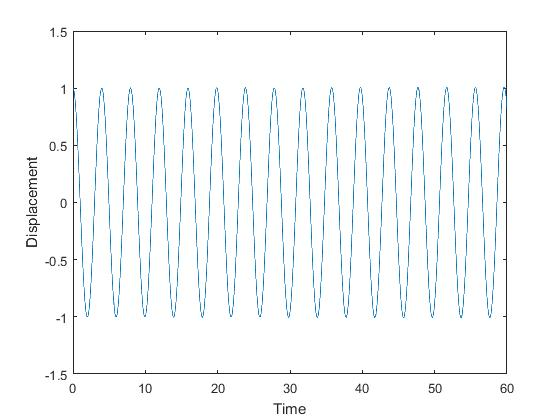
\includegraphics[width=0.9\textwidth]{4}
		\caption{First order Forward Euler time-displacement graph (at a very low time step).}
	\end{figure} 
	\newpage
	\part*{5}
	The program does not pass the test at high values for the time step. I noticed that in this case, the position of the spring will actually gradually increase further above the initial position, which is not correct according to the law of momentum. The test criterion made sense, however the algorithm does not accommodate the momentum law and other physics laws such as friction (the latter of which would actually cause the spring to slow down gradually until it reaches equilibrium).
	\part*{6}
	The function E(t) seems to be fairly linear, along the lines of E(t) = 2.5. Please refer to the file ex\_6.m for the calculation of the energy at each time step. When plotting the energy at a high value for the time step, the energy will increase over time, as the amplitude of the swing also increases. Again, this is the major flaw of this algorithm.
	\begin{figure}[!ht]
		\centering
		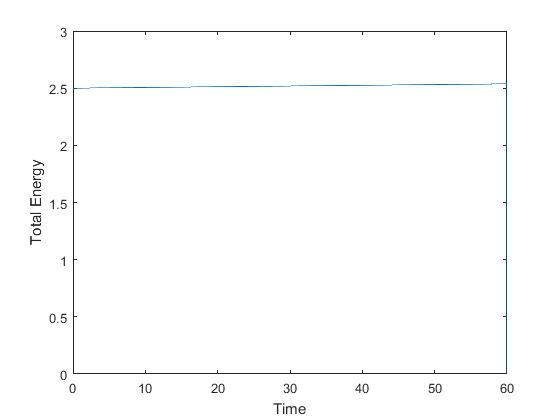
\includegraphics[width=0.9\textwidth]{6}
		\caption{First order Forward Euler time-energy graph.}
	\end{figure}
	\part*{7}
	See file ex\_7.m. The amount of energy in the system is now linear. The inaccuracy of the Euler scheme seems to have been solved by using this leap-frog version of the Verlet algorithm.
	\begin{figure}[!ht]
		\centering
		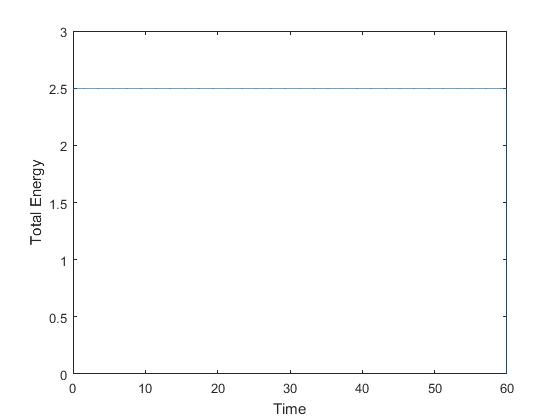
\includegraphics[width=0.9\textwidth]{7}
		\caption{Verlet leap-frog time-energy graph.}
	\end{figure}
	\part*{8}
	The interpretation of the velocity causes a change in the calculation of the total energy in the system:\\\\
	$E(t) = E(k) + E(p) = (1/2)mv^2 + (1/2)kx^2$\\\\
	Overall, this change seems to bring more balance into the equation as a whole.
	\part*{9}
	For the two Taylor expansions, we have:\\\\
	$x(t+\Delta t) = x(t) + \dot{x}(t)\Delta t + (1/2)\ddot{x}(t)\Delta t^2+(1/6)\dddot{x}(t)\Delta t^3+O(\Delta t^4)$\\
	and\\
	$x(t-\Delta t) = x(t) - \dot{x}(t)\Delta t  + (1/2)\ddot{x}(t)-\Delta t^2+(1/6)\dddot{x}(t)-\Delta t^3+O(\Delta t^4)$\\\\
	Adding these two Taylor expansions leads to the following solution for the Verlet algorithm:\\
	$x(t+\Delta t) + x(t-\Delta t) = 2x(t)+\ddot{x}(t)(\Delta t^2) + O(\Delta t^4)$.\\\\
	As for the comparison to Equation (1), $d^2x(t)/\Delta t^2 = F(x(t))/m$, this constitutes the following: $d^2x(t)/\Delta t^2$ is the acceleration of the spring at time t.\\\\
	First, we solve w[i] from Eq. 6:\\
	$x[i+1] = x[i] + w[i+1]*\Delta t =$\\
	$x[i+1] = x[i] + (w[i] + a*\Delta t)*\Delta t =$\\
	$x[i+1] = x[i] + w[i]*\Delta t + a*\Delta t^2$\\
	$w[i] = (x[i+1]-x[i]-a*\Delta t^2)/\Delta t$\\\\
	Next, we insert w[i] into the calculation for w[i+1]:\\
	$w[i+1] = (x[i+1]-x[i]-a*\Delta t^2)/\Delta t + a*\Delta t$\\
	$w[i+1] = (x[i+1] - x[i])/\Delta t$
	
	The local truncation error equals O($\Delta$$t^4$), as has been derived from adding the two Taylor expansions.
	\newpage
	\part*{10}
	The time step is determined by the algorithm, the only thing that has to be done is the definition of a start and end time.
	\begin{figure}[!ht]
		\centering
		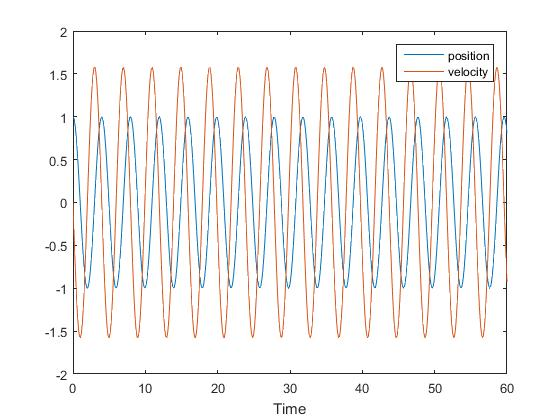
\includegraphics[width=0.9\textwidth]{10}
		\caption{ODE45 time-displacement/velocity graph.}
	\end{figure}
	\newpage
	\part*{11}
	In terms of accuracy and long-time stability, the leap-frog version of Verlet's algorithm seems to be performing the best out of all three. Its energy plot stays at the same height regardless of the simulation length, which is what we would expect (conservation of energy because there is no friction/damping involved). The energy plot for the ODE45 algorithm can be found in the file ex\_11.m.
	\begin{figure}[!ht]
		\centering
		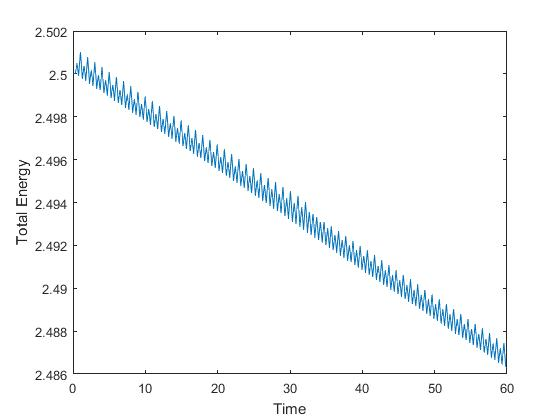
\includegraphics[width=0.9\textwidth]{11}
		\caption{ODE45 time-energy graph.}
	\end{figure}
	\part*{12}
	We can include the friction force in the ODE45 algorithm by inputting it into the derivation function:\\\\
	$dxdt = (-k * p - c * v)/m$\\
	where p is the position of the system and c is the friction parameter.\\\\
	We can include the friction force into the leap-frog algorithm by inserting the friction coefficient into the calculation of the new speed.
	The consequence for the integration scheme is that the function will slowly decay over time.
	\part*{13}
	Please refer to enclosed files ex\_13.m and harmonic\_oscillator\_damped.m. The figure below shows the decay in the energy of the swing. As the oscillation reaches its equilibrium, neither kinetic nor potential energy will be present anymore. Therefore, the total energy in the system will slowly go towards zero.
	\begin{figure}[!ht]
		\centering
		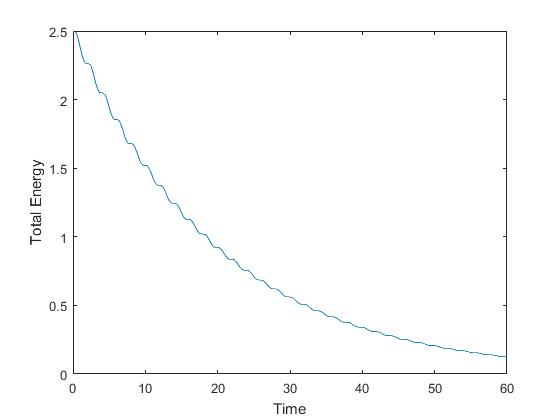
\includegraphics[width=0.9\textwidth]{13}
		\caption{ODE45 damped time-energy graph.}
	\end{figure}
	\part*{14}
	We can introduce a driving force into the ode45 algorithm by inputting it into the derivation function as we did with the friction force:\\\\
	$dxdt = (-k * p - c * v + f * cos(\omega * t))/m)$.\\
	where $\omega$ is the frequency and f is the amplitude of the driving force.\\\\
	\part*{15}
	Please refer to enclosed files ex\_15.m and harmonic\_oscillator\_damped\_driven.m. The main observation that can be made from the resulting graph, is that the driving force activates every so often, causing a brief rise in energy. Eventually, the spring will still slowly reach equilibrium, and the energy will therefore still go towards zero.
	\begin{figure}[!ht]
		\centering
		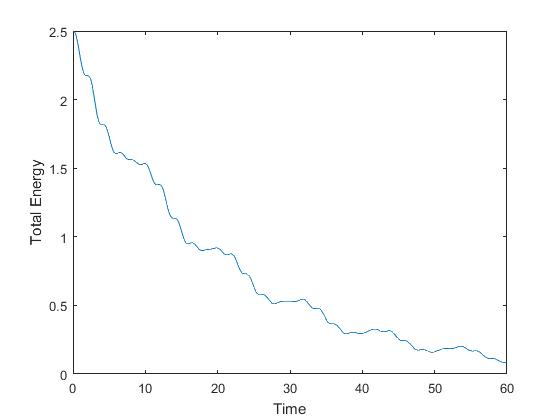
\includegraphics[width=0.9\textwidth]{15}
		\caption{ODE45 damped and driven time-energy graph.}
	\end{figure}
\end{document}